\documentclass{article}
\usepackage[T1]{fontenc}
\usepackage[croatian]{babel}
\usepackage[left=25mm,right=25mm,top=25mm,bottom=25mm,paper=a4paper]{geometry}
\usepackage{graphicx}
\usepackage{enumitem}
\usepackage{float}
\usepackage{fancyhdr}
\pagestyle{fancy}
\usepackage{hyperref}
\graphicspath{{Slike/}}
\fancyhf{}





\title{Konfiguracija Osobnog Računala}
\author{Dominik Jurusic}
\date{\today}

\begin{document}

\maketitle
\tableofcontents
\listoffigures
\pagebreak



\section{Svrha Računala}
Ovo gaming računalo pruža strastvenim igračima vrhunske performanse s AMD Ryzen 7 5800X3D procesorom i RX 6600XT grafičkom karticom. S brzim NVMe SSD-om i prostranim Toshiba HDD-om omogućuje brzo učitavanje igara i obilje prostora za pohranu. Sa Corsair 16GB RAM-om pruža odzivnu memoriju za multitasking, dok estetski dizajn s RGB osvjetljenjem doprinosi gaming atmosferi. Ovo računalo je stvoreno kako bi pružilo nezaboravno iskustvo igranja u natjecateljskim borbama ili uživanju u najnovijim blockbuster igrama.

\section{Komponente}

\subsection{Procesor (CPU)}
\begin{figure}[H]
    \centering
    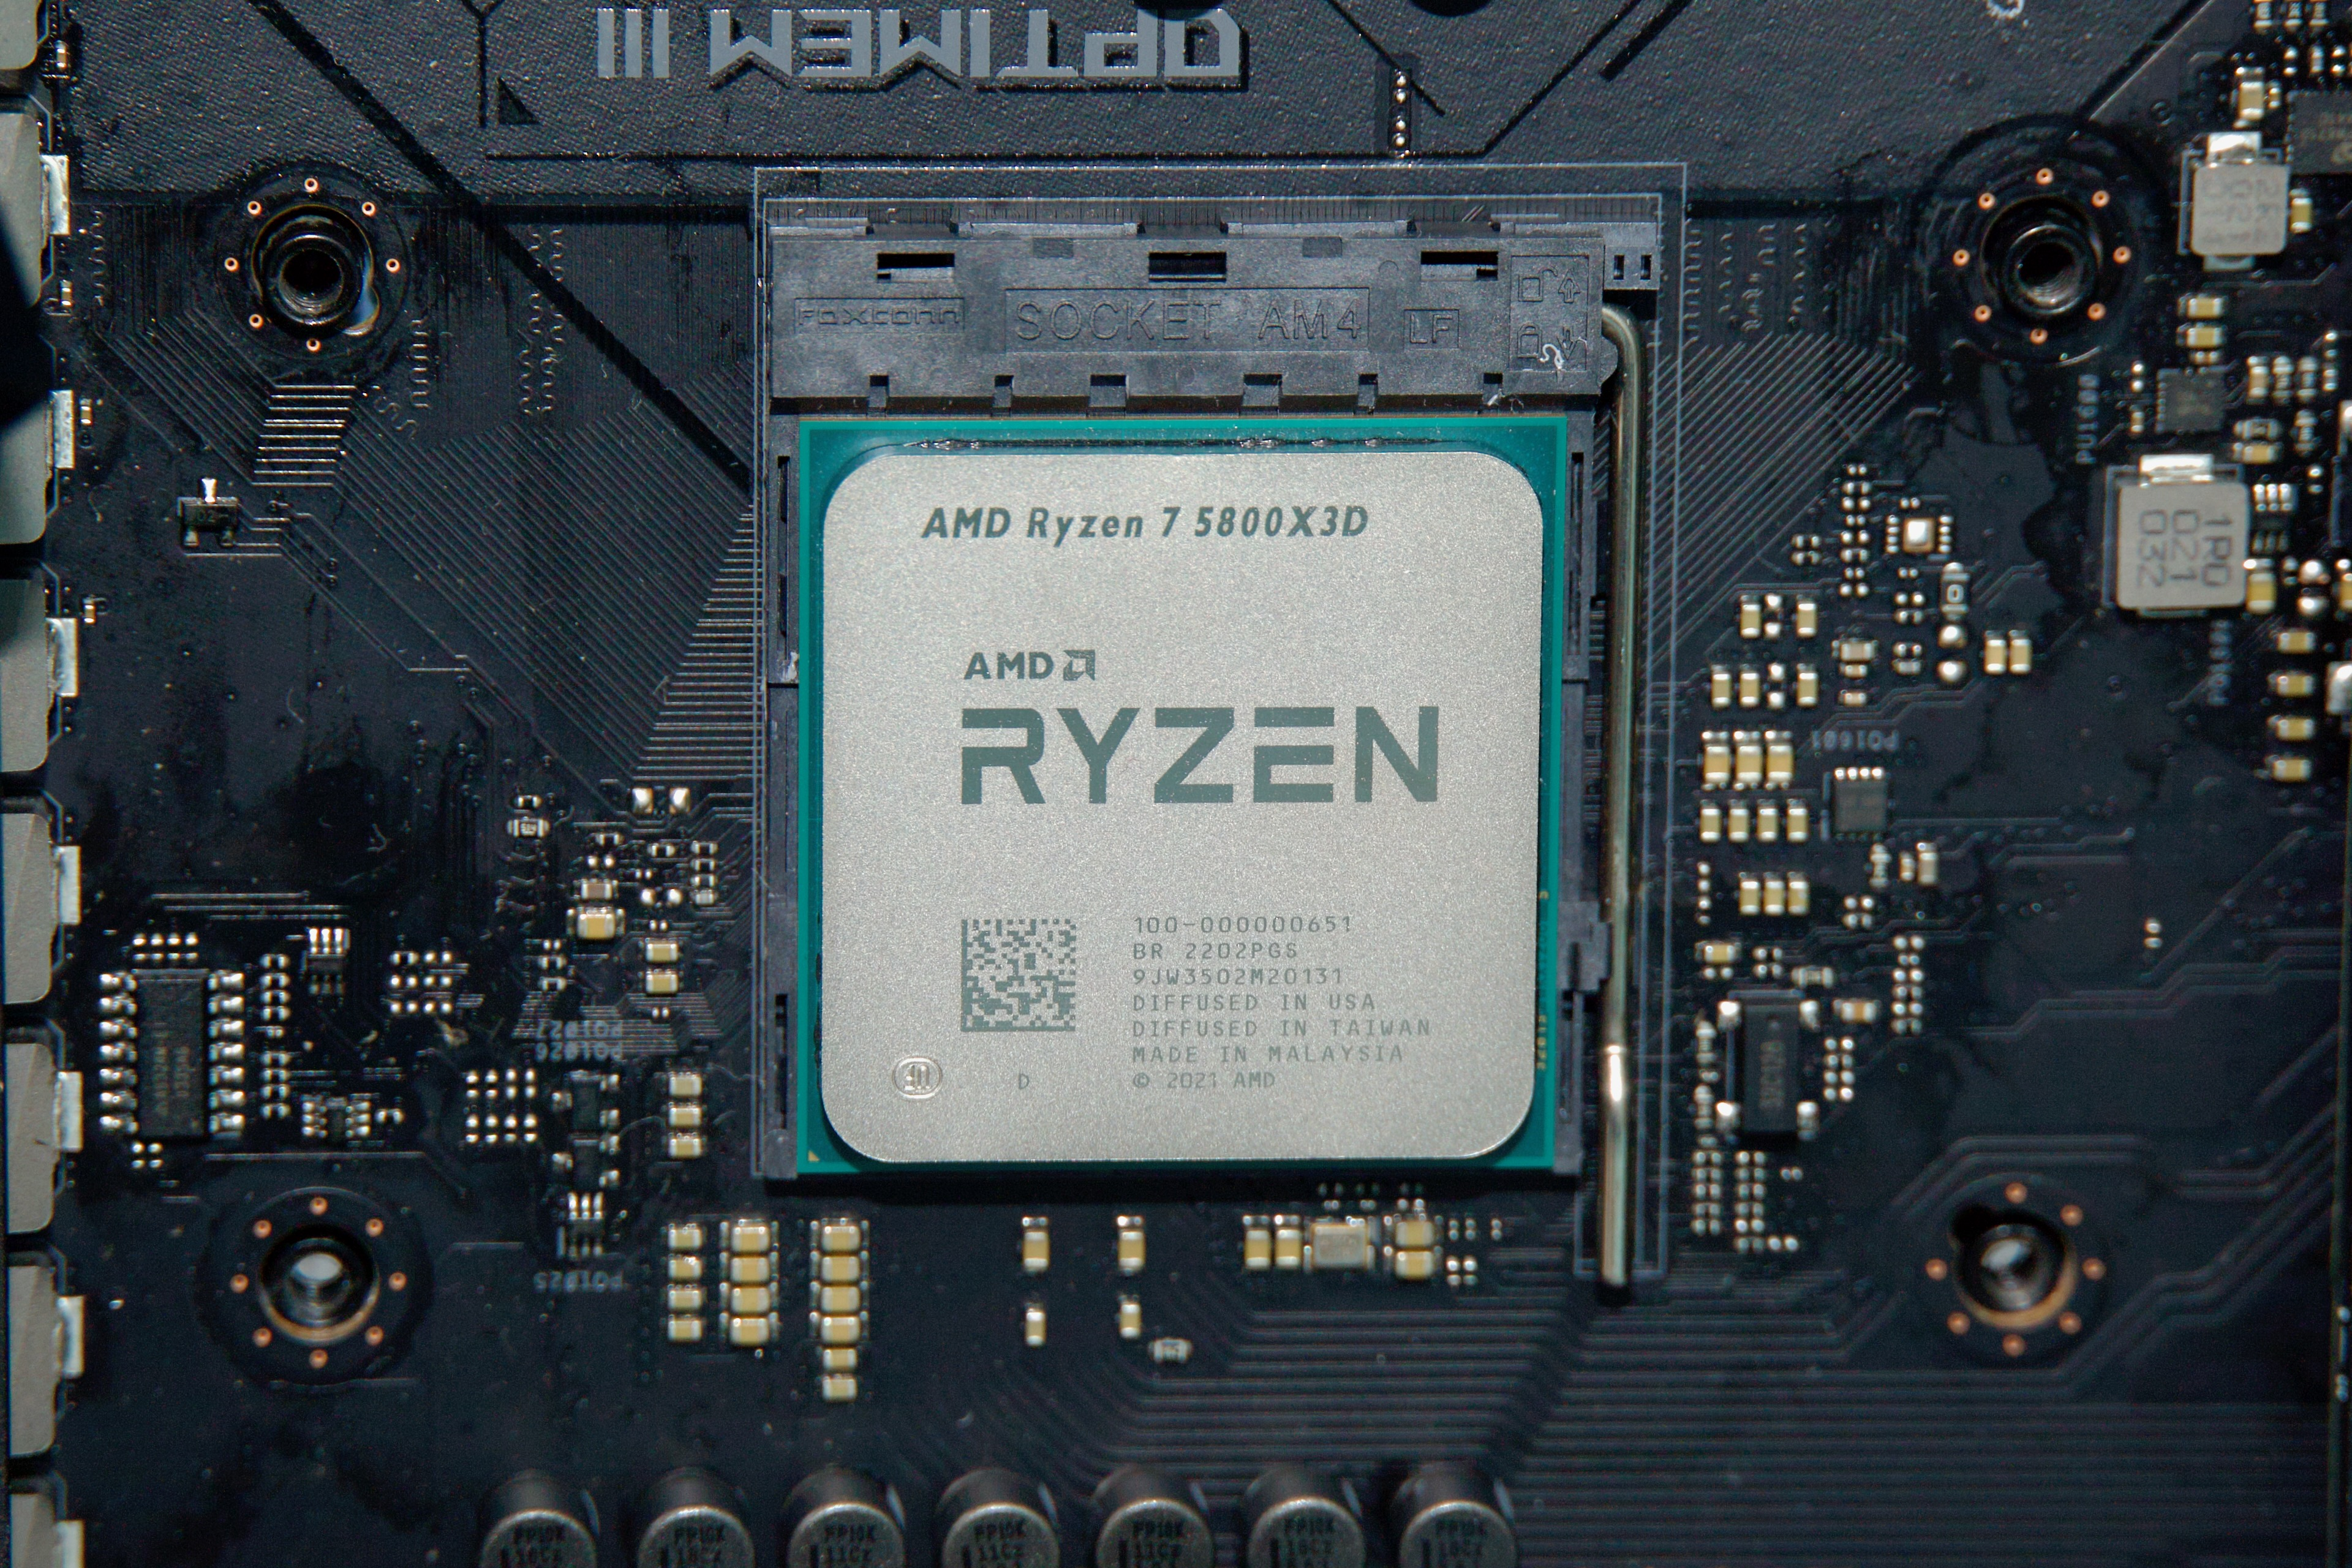
\includegraphics[width = \textwidth]{Slike/CPU.jpg}
    \caption{AMD Ryzen 7 5800X3D}
    \label{fig:Procesor}
\end{figure}
\begin{itemize}
    \item Model: Ryzen 7 5800x3d
    \item Brzina: 3.4 GHz (base), 4.5 GHz (boost)
    \item Broj jezgara: 8, Broj dretvi: 16
    \item Obrazloženje: Odabran zbog visokih performansi 
    \item Cijena: 370 EUR (\href{https://www.adm.hr/cpu-amd-ryzen-7-5800x3d-box-am4-100-100000651wof/72892/product/}{Shop})
\end{itemize}

\subsection{Grafička kartica}
\begin{figure}[H]
    \centering
    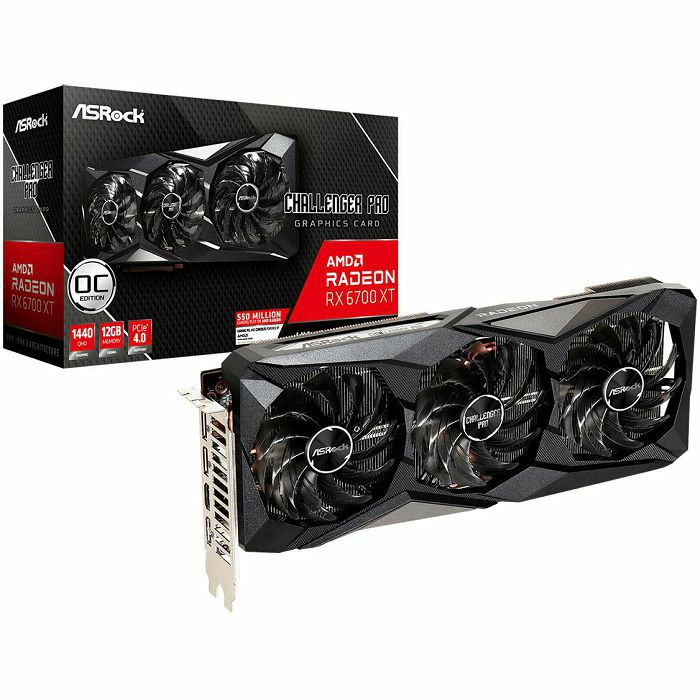
\includegraphics[width = \textwidth]{Slike/graficka.jpg}
    \caption{AMD RX 6600XT}
    \label{fig:Grafička kartica}
\end{figure}
\begin{itemize}
    \item Model: AMD RX 6600XT
    \item Grafički procesor: RDNA 2
    \item Stream Processors: 2048
    \item Brzina GPU-a: Do 2589 MHz
    \item VRAM: 8GB GDDR6
    \item Sučelje: PCIe 4.0
    \item Dodatne značajke: Ray Tracing, FidelityFX Super Resolution (FSR)
    \item Obrazloženje: AMD RX 6600XT je odabran zbog izvrsnih performansi i podrške za suvremene grafičke tehnologije poput Ray Tracinga i FSR-a.
    \item Cijena: 412 EUR (\href{https://tehno-mag.hr/graficka-kartica-msi-rx-6600-xt-8gb-mech-2x-oc-proizvod-8005/}{Shop})
\end{itemize}
\pagebreak


\subsection{Matična ploča}
\begin{figure}[H]
    \centering
    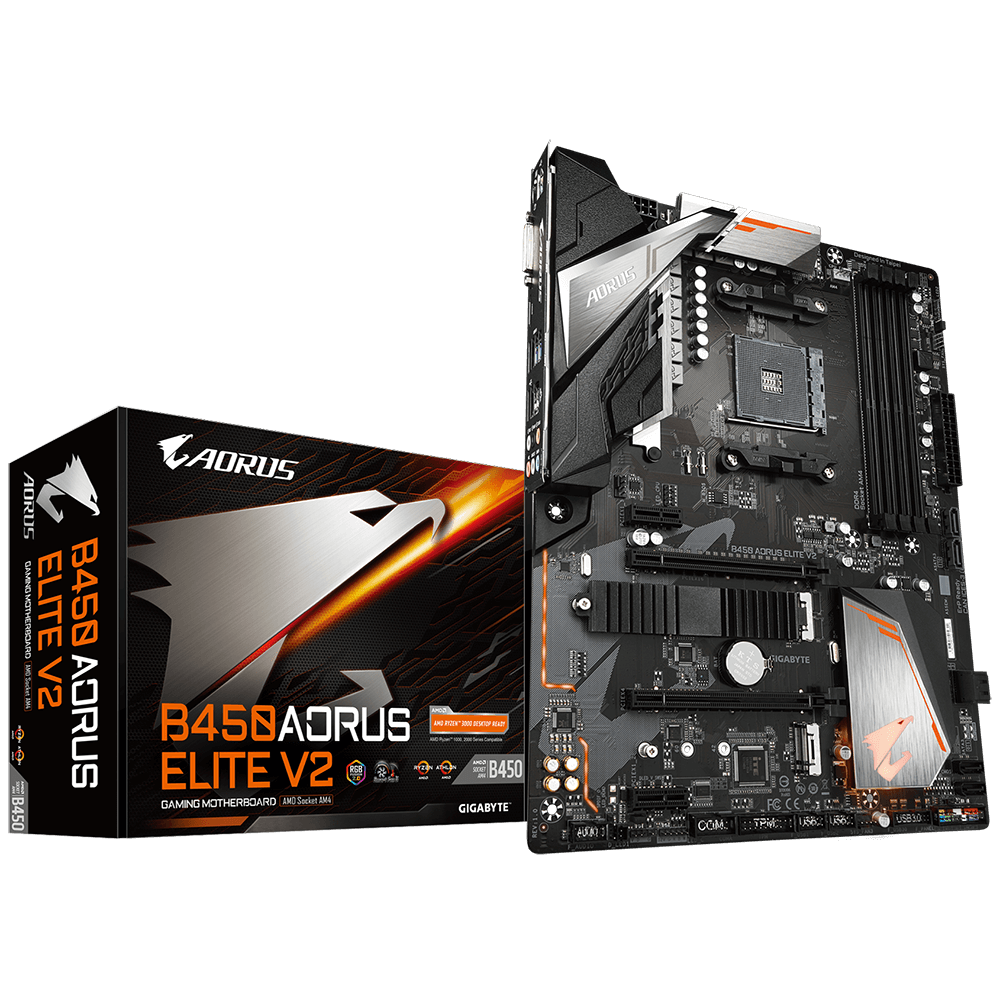
\includegraphics[width = \textwidth]{Slike/Maticna.jpg}
    \caption{B450 AORUS ELITE v2}
    \label{fig:Matična}
\end{figure}
\begin{itemize}
    \item Model: B450 AORUS Elite
    \item Čipset: AMD B450
    \item Podrška za procesore: AMD Ryzen serije 3000
    \item PCIe 3.0, M.2 sučelja, USB 3.1
    \item Audio: Realtek ALC1200
    \item LAN: Intel GbE LAN
    \item Obrazloženje: B450 AORUS Elite pruža stabilnu platformu za AMD Ryzen procesore s odgovarajućim sučeljima i funkcijama potrebnim za rad s odabranim komponentama.
    \item Cijena: 102 EUR (\href{https://laptopi.hr/informatika/komponente/maticne-ploce/motherboard-b450-aorus-elite-v2-am4-4ddr4-dvi-hdmi-m-2-atx-detail?utm_source=nabava.net&utm_campaign=nabava.net&utm_medium=click}{Shop})
\end{itemize}

\subsection{RAM memorija}
\begin{figure}[H]
    \centering
    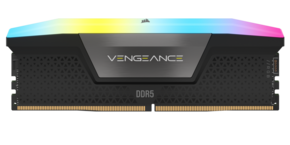
\includegraphics[width = \textwidth]{Slike/ram.jpg}
    \caption{Corsair Vengeance LPX}
    \label{fig:RAM}
\end{figure}
\begin{itemize}
    \item Model: Corsair Vengeance LPX
    \item Kapacitet: 2x8GB
    \item Brzina: 3000MHz
    \item Tip: DDR4
    \item CAS Latencija: CL16
    \item Obrazloženje: Corsair Vengeance LPX pruža pouzdanu i brzu radnu memoriju koja podržava visoke performanse sustava, a odabrana je zbog ravnoteže između brzine i pouzdanosti.
    \item Cijena: 26*2 EUR (\href{https://laptopi.hr/informatika/komponente/memorije-1/ddr4-vengeance-lpx-8gb-3000-1-8gb-black-cl16-detail?utm_source=nabava.net&utm_campaign=nabava.net&utm_medium=click}{Shop})
\end{itemize}


\subsection{Tvrdi Disk (HDD)}
\begin{figure}[H]
    \centering
    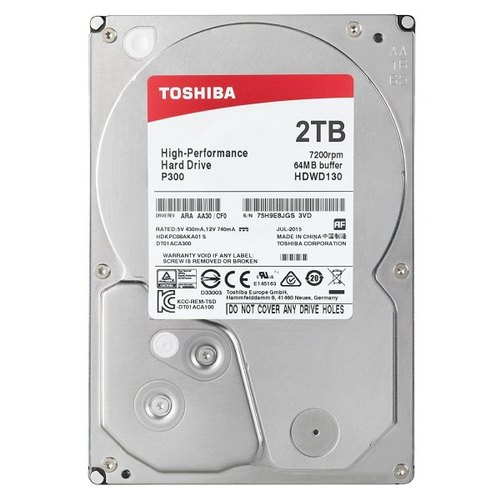
\includegraphics[width = \textwidth]{Slike/HDD.jpg}
    \caption{Hard disk}
    \label{fig:HDD}
\end{figure}
\begin{itemize}
    \item Model: Toshiba 2TB HDD
    \item Kapacitet: 2TB
    \item Brzina vrtnje: 7200 RPM
    \item Cache: 256MB
    \item Sučelje: SATA3
    \item Obrazloženje: Toshiba 2TB HDD pruža dodatni prostor za pohranjivanje podataka i aplikacija koje ne zahtijevaju veliku brzinu.
    \item Cijena: 67 EUR (\href{https://www.adm.hr/toshiba-2tb-35-7200rpm-256mb-p300-hdwd320uzsva/76518/product/?utm_source=nabava.net&utm_campaign=nabava.net&utm_medium=click}{Shop})
\end{itemize}
\pagebreak

\subsection{NVME ssd}
\begin{figure}[H]
    \centering
    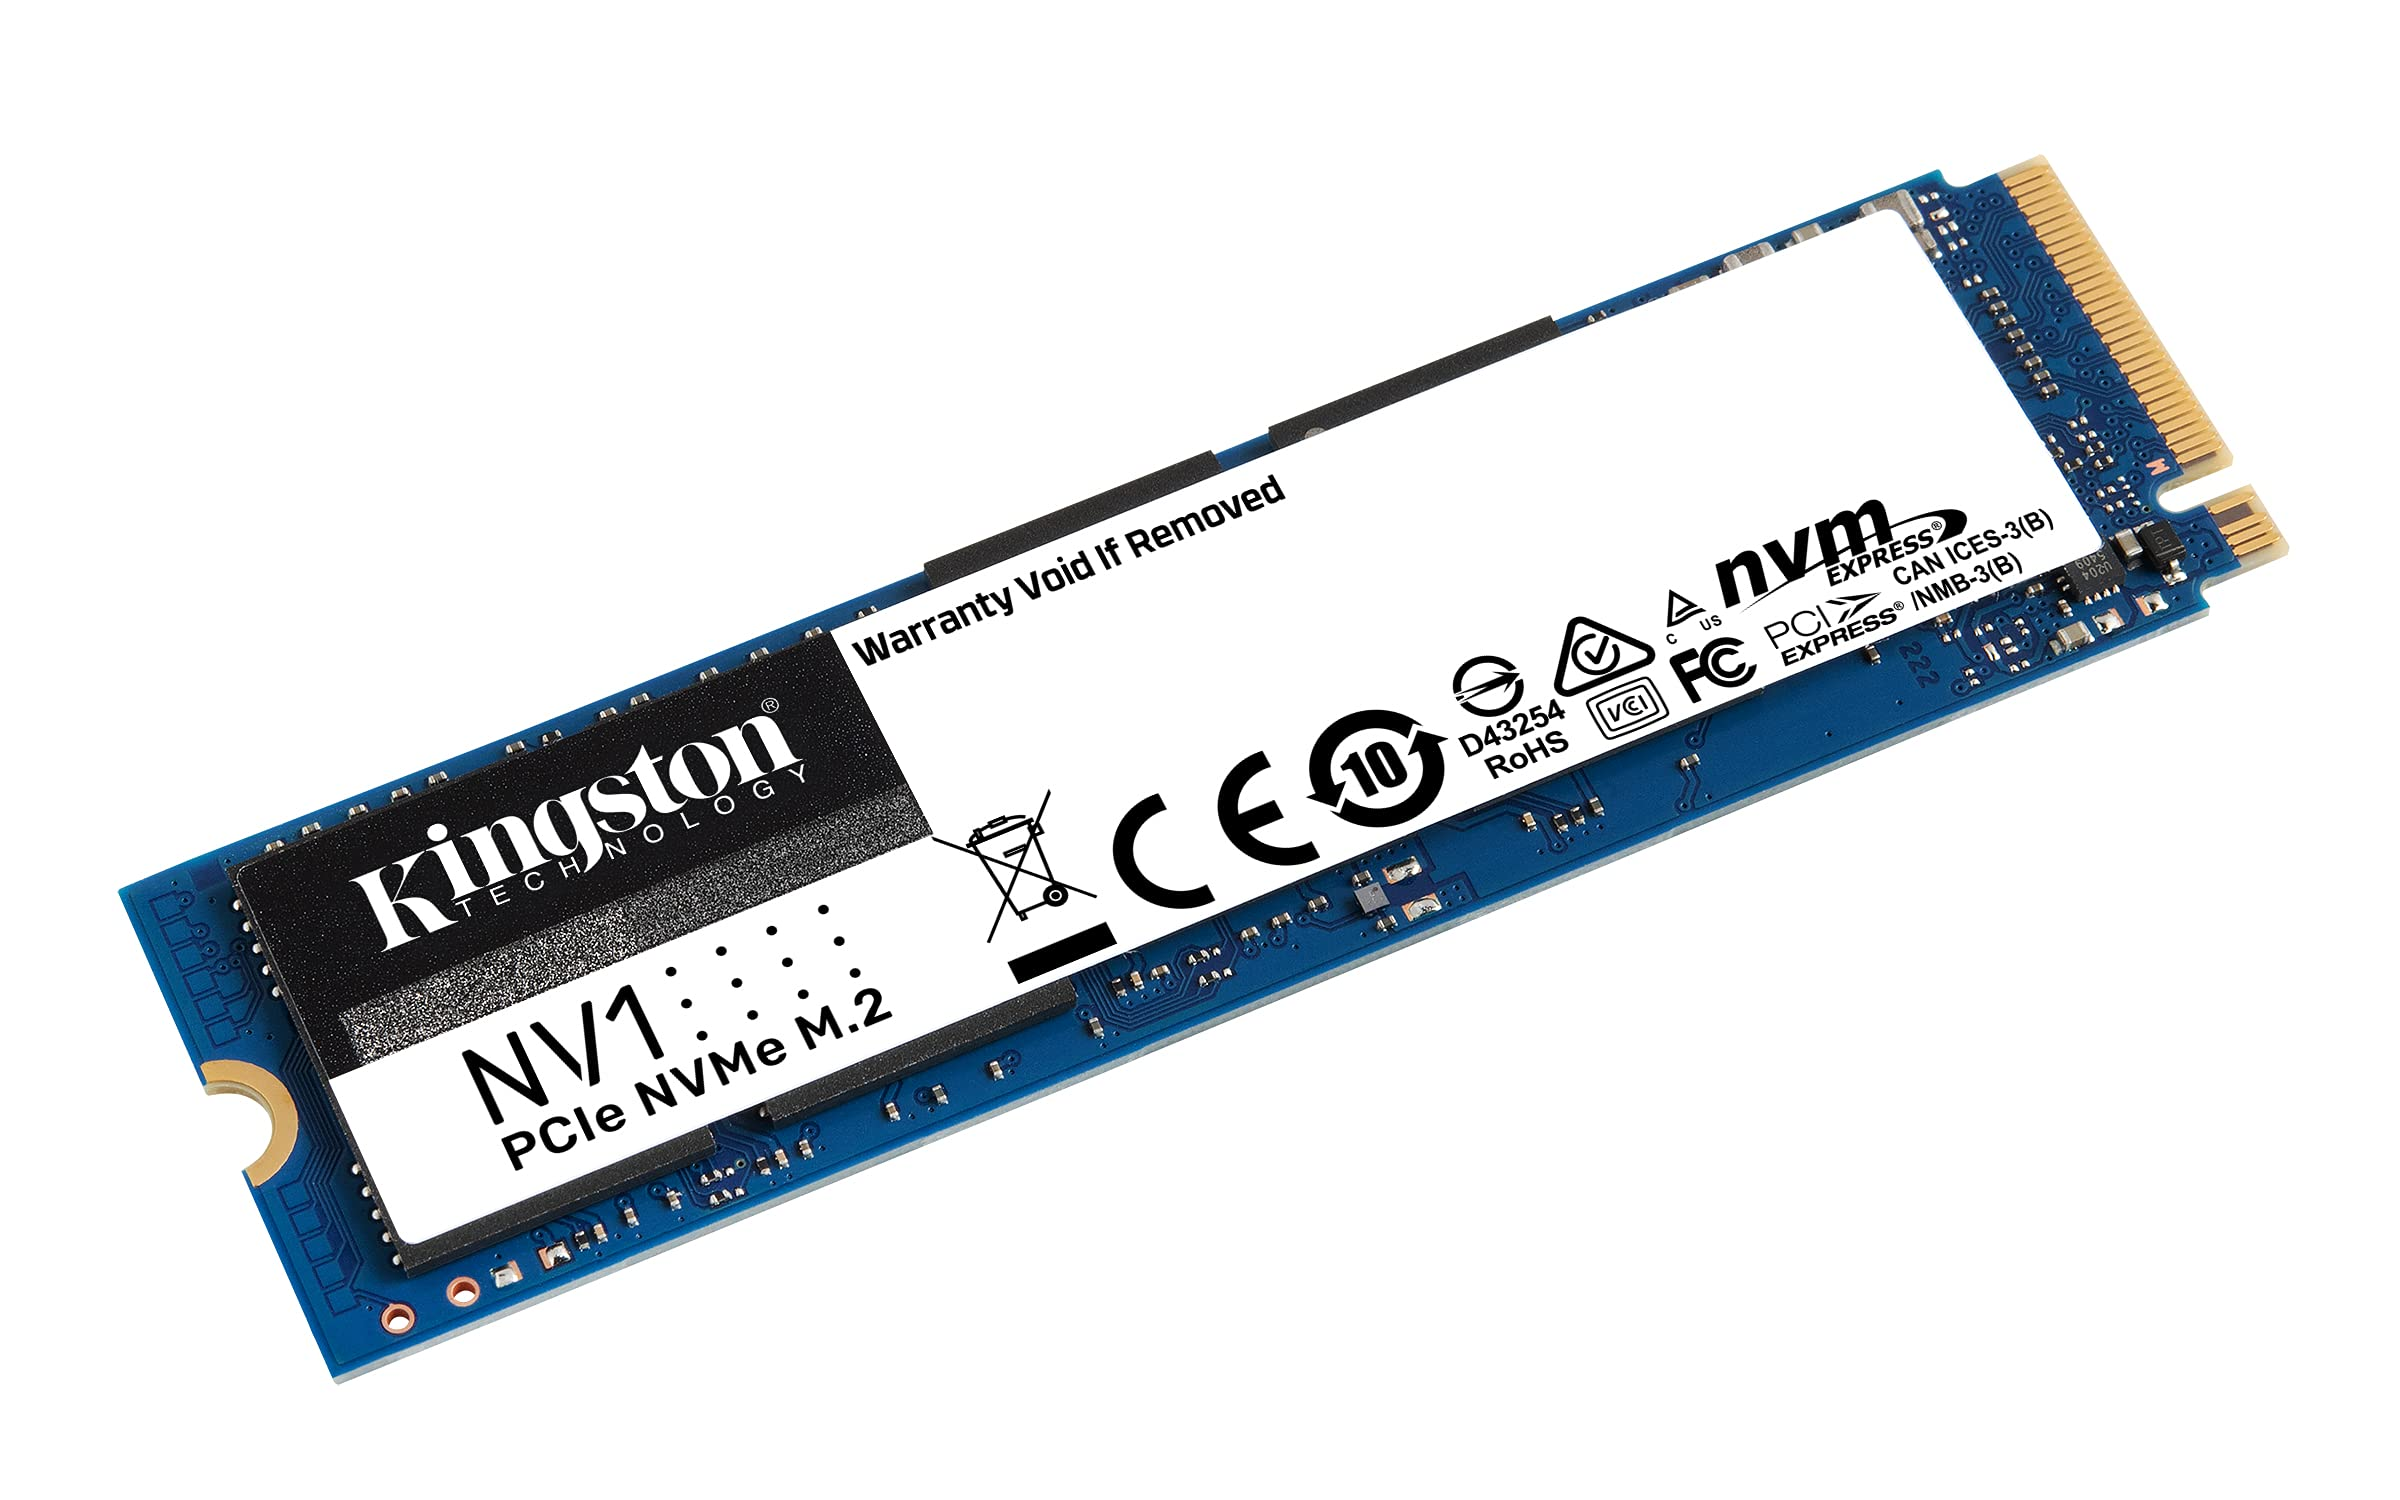
\includegraphics[width = \textwidth]{Slike/NVMe.jpg}
    \caption{Kingston NV1 1TB M.2 2280 NVMe}
    \label{fig:NVMe}
\end{figure}
\begin{itemize}
    \item Model: Kingston NV1 1TB M.2 2280 NVMe
    \item Kapacitet: 1TB
    \item Sučelje: M.2 2280, NVMe
    \item Brzina čitanja: Do 2,100 MB/s
    \item Brzina pisanja: Do 1,700 MB/s
    \item Obrazloženje: Kingston NV1 1TB pruža brze prijenose podataka zahvaljujući NVMe sučelju, čineći ga odličnim izborom za brzo učitavanje igara i ima puno prostora za pohranu.
    \item Cijena: 95 EUR (\href{https://vacom.hr/proizvod/ssd-kingston-nv1-1tb-m-2-2280-nvme/}{Shop})
\end{itemize}


\subsection{PSU}
\begin{figure}[H]
    \centering
    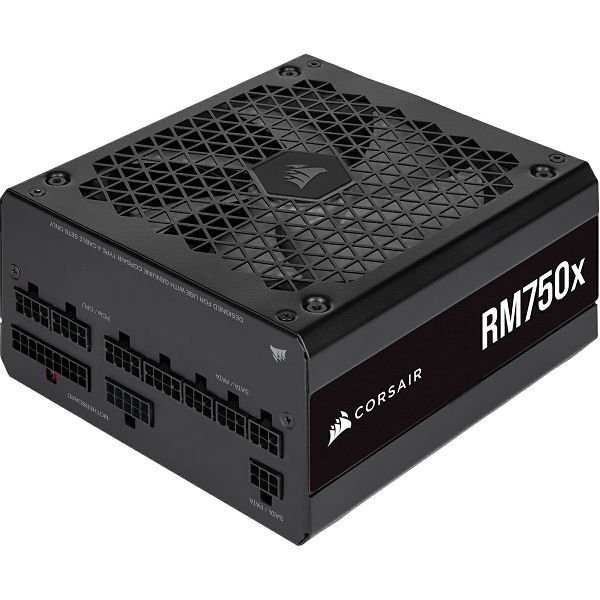
\includegraphics[width = \textwidth]{Slike/PSU.jpg}
    \caption{Power supply}
    \label{fig:PSU}
\end{figure}
\begin{itemize}
    \item Model: Corsair RM750x, 750W, 80 PLUS Gold
    \item Snaga: 750W
    \item Certifikacija: 80 PLUS Gold
    \item Modularnost: modularno napajanje
    \item Ventilator: 135mm 
    \item Dodatne značajke: tiho je, Corsair LINK kompatibilnost
    \item Obrazloženje: Corsair RM750x pruža dovoljno snage za pokretanje konfiguracije i ima visok stupanj učinkovitosti s 80 PLUS Gold certifikatom. Laka organizacija kablova i nivo buke je nizak.
    \item Cijena: 183 EUR (\href{https://www.instar-informatika.hr/napajanje-corsair-rm750x-750w-80-gold-modularno-atx/103917/product/}{Shop})
\end{itemize}

\pagebreak

\section{Periferija}

\subsection{Monitor}
\begin{figure}[H]
    \centering
    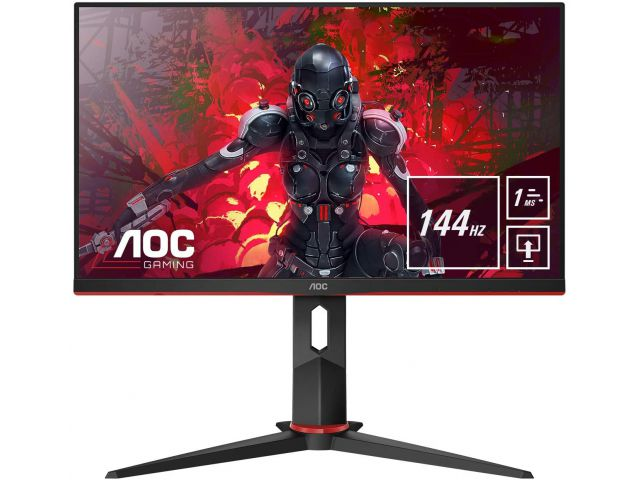
\includegraphics[width = \textwidth]{Slike/Monitor.jpg}
    \caption{Monitor}
    \label{Slika:monitor}
\end{figure}
\begin{itemize}
    \item Model: AOC 24G2U
    \item Veličina zaslona: 24"
    \item Tehnologija zaslona: IPS 
    \item Rezolucija: 1920x1080 
    \item Vrijeme odziva: 1ms
    \item Frekvencija: 144 Hz
    \item Portovi: DisplayPort, 2x HDMI
    \item USB priključci: 4x USB 3.0
    \item Zvučnici: Ugrađeni zvučnici
    \item Obrazloženje: Ovaj monitor ima malo vrijeme odaziva i veću frekvenciju što je jako korisno za Gaming
    \item Cijena: 200 EUR (\href{https://www.hgspot.hr/monitor-aoc-24g2u-24-ips-fhd-1920x1080px-1ms-144-hz-dp-2x-hdmi-amd-freesync-4x-usb3-0-zvucnici}{Shop})
\end{itemize}


\subsection{Miš}
\begin{figure}[H]
    \centering
    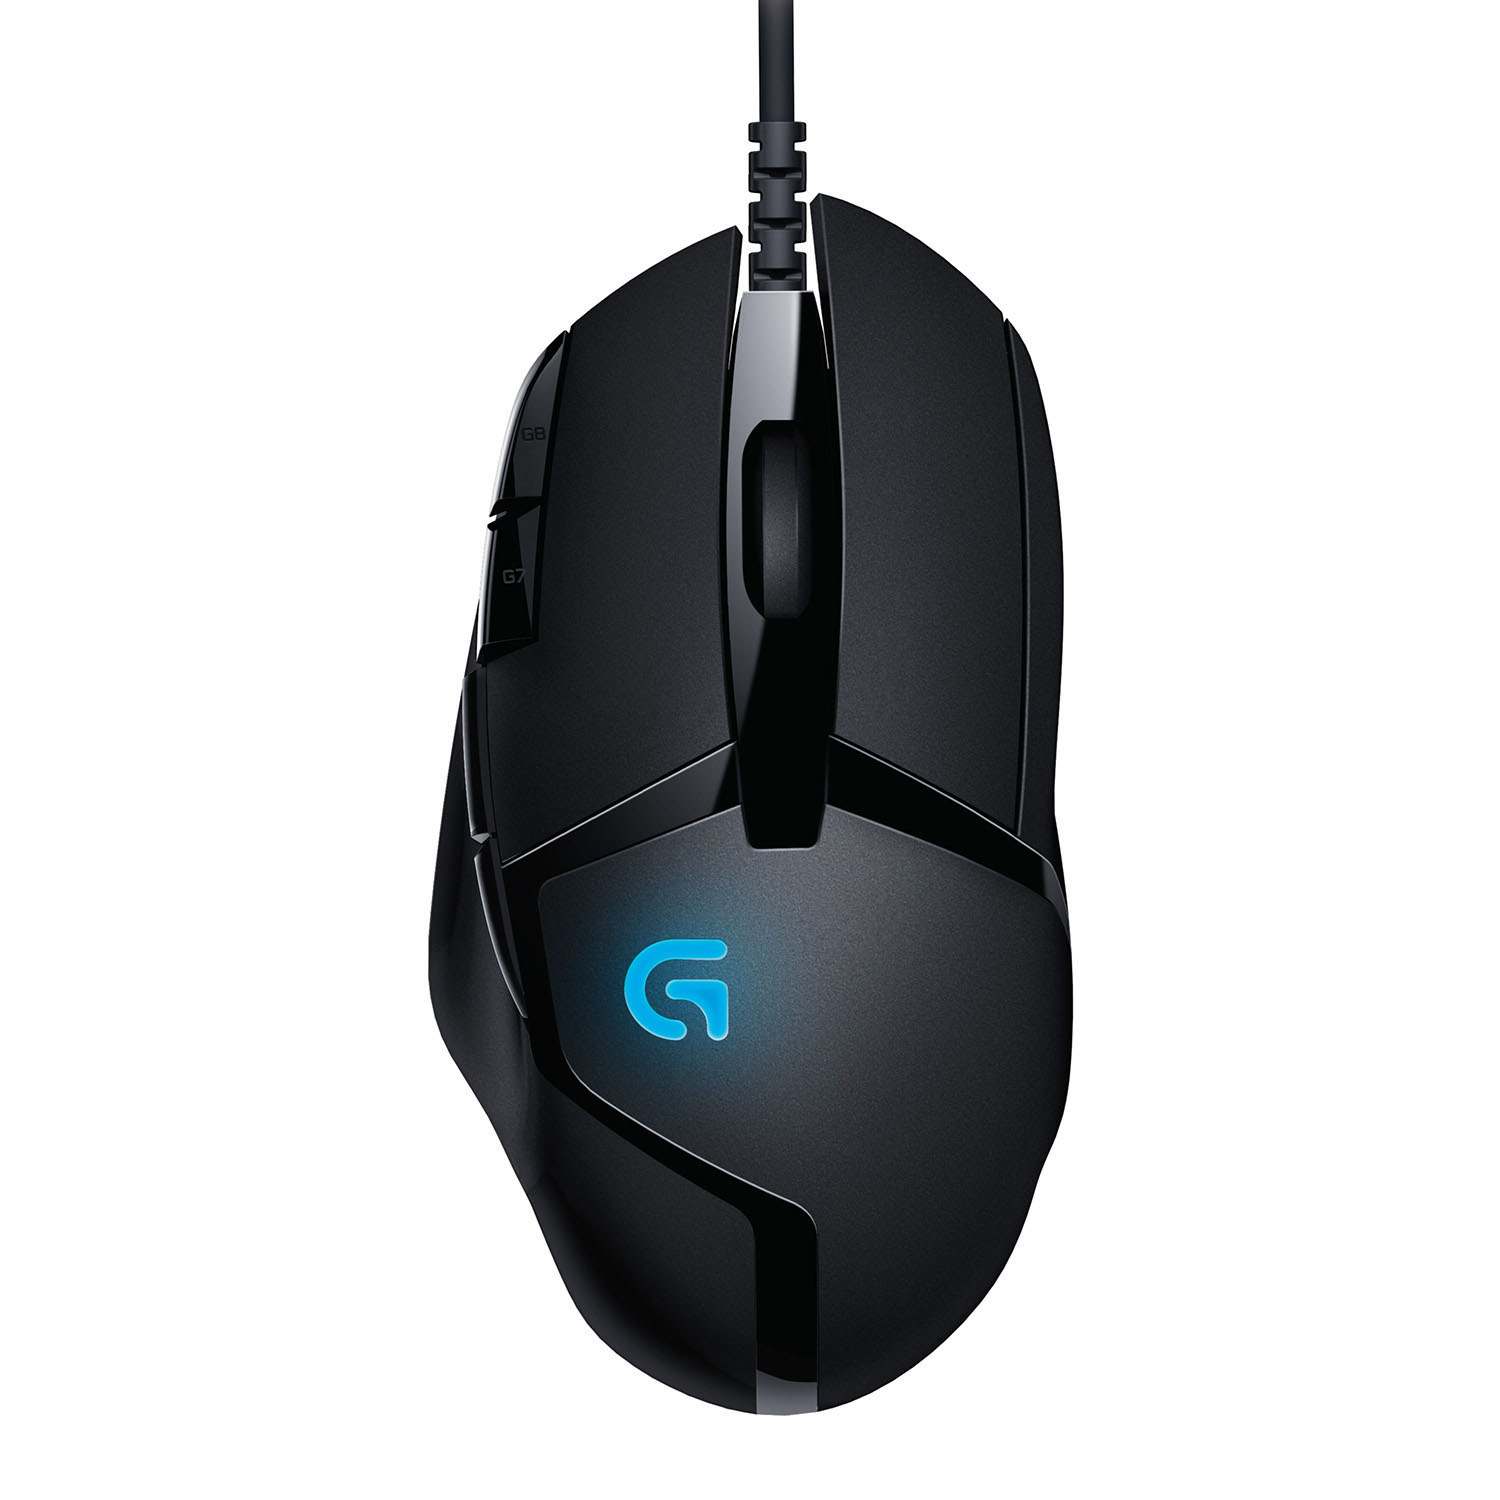
\includegraphics[width = \textwidth]{Slike/G402.jpg}
    \caption{Miš}
    \label{fig:Miš}
\end{figure}
\begin{itemize}
    \item Model: Logitech G402 Hyperion Fury
    \item Senzor: Optički, Fusion Engine
    \item DPI (dots per inch): 240 - 4000 DPI
    \item Brzina praćenja: 500 ips
    \item Broj tipki: 8 programabilnih tipki
    \item Frekvencija osvježavanja : 1ms (1000Hz)
    \item Mikroprocesor: 32-bitni
    \item Osvjetljenje: LED, podesivo
    \item Dodatne značajke: On-the-Fly DPI promjena
    \item Obrazloženje: Logitech G402 Hyperion Fury odabran je zbog svoje preciznosti i brzine, ključnih aspekata za gaming iskustvo.
    \item Cijena: 70 EUR (\href{https://www.links.hr/hr/mis-logitech-gaming-g402-hyperion-fury-deltazero-4000dpi-crni-usb-101503412}{Shop})
\end{itemize}


\subsection{Tipkovnica}
\begin{figure}[H]
    \centering
    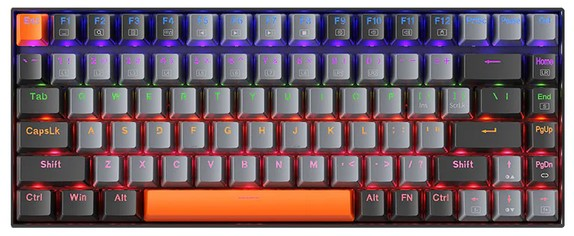
\includegraphics[width = \textwidth]{Slike/Tipkovnica..jpg}
    \caption{Tipkovnica}
    \label{fig:Tipkovnica}
\end{figure}
\begin{itemize}
    \item Model: K500A-B84
    \item Tip switcha: Mehanički, red
    \item Izdržljivost switcha: Do 50 milijuna pritisaka
    \item Pozadinsko osvjetljenje: RGB.
    \item Materijal kućišta: Aluminijsko kućište
    \item Sila aktivacije switcha: 45g
    \item Udaljenost na kojoj se priznaje input switcha: 2.4mm
    \item Udaljenost na kojoj switch dolazi do dna tipkovnice: 4.4mm
    \item Obrazloženje: Tipkovnica je jako responzivna i brza za tipkanje što je jako dobro za svaki posao koji zahtijeva puno tipkanja ili za gaming.
    \item Cijena: 32 EUR (\href{https://www.aliexpress.com/item/1005005958708733.html?spm=a2g0o.order_list.order_list_main.5.51111802yyqjTU}{Shop})
\end{itemize}

\section{Ukupna Cijena}
\begin{itemize}
    \item lorem ipsum
\end{itemize}

\section{Zaključak}
lorem ipsum     

\end{document}
